\documentclass[man, fleqn, noextraspace]{apa6}
\usepackage{lmodern}
\usepackage{amssymb,amsmath}
\usepackage{ifxetex,ifluatex}
\usepackage{fixltx2e} % provides \textsubscript
\ifnum 0\ifxetex 1\fi\ifluatex 1\fi=0 % if pdftex
  \usepackage[T1]{fontenc}
  \usepackage[utf8]{inputenc}
\else % if luatex or xelatex
  \ifxetex
    \usepackage{mathspec}
  \else
    \usepackage{fontspec}
  \fi
  \defaultfontfeatures{Ligatures=TeX,Scale=MatchLowercase}
\fi
% use upquote if available, for straight quotes in verbatim environments
\IfFileExists{upquote.sty}{\usepackage{upquote}}{}
% use microtype if available
\IfFileExists{microtype.sty}{%
\usepackage{microtype}
\UseMicrotypeSet[protrusion]{basicmath} % disable protrusion for tt fonts
}{}
\usepackage{hyperref}
\hypersetup{unicode=true,
            pdftitle={A Comparative Analysis on Native and Non-Native Korean Speakers' Vowel Productions},
            pdfauthor={Jungah-Lee, Heidi Shi, \& Jeongim Jin},
            pdfkeywords={Korean Vowels, L1 Phonetics},
            pdfborder={0 0 0},
            breaklinks=true}
\urlstyle{same}  % don't use monospace font for urls
\usepackage{graphicx,grffile}
\makeatletter
\def\maxwidth{\ifdim\Gin@nat@width>\linewidth\linewidth\else\Gin@nat@width\fi}
\def\maxheight{\ifdim\Gin@nat@height>\textheight\textheight\else\Gin@nat@height\fi}
\makeatother
% Scale images if necessary, so that they will not overflow the page
% margins by default, and it is still possible to overwrite the defaults
% using explicit options in \includegraphics[width, height, ...]{}
\setkeys{Gin}{width=\maxwidth,height=\maxheight,keepaspectratio}
\IfFileExists{parskip.sty}{%
\usepackage{parskip}
}{% else
\setlength{\parindent}{0pt}
\setlength{\parskip}{6pt plus 2pt minus 1pt}
}
\setlength{\emergencystretch}{3em}  % prevent overfull lines
\providecommand{\tightlist}{%
  \setlength{\itemsep}{0pt}\setlength{\parskip}{0pt}}
\setcounter{secnumdepth}{0}
% Redefines (sub)paragraphs to behave more like sections
\ifx\paragraph\undefined\else
\let\oldparagraph\paragraph
\renewcommand{\paragraph}[1]{\oldparagraph{#1}\mbox{}}
\fi
\ifx\subparagraph\undefined\else
\let\oldsubparagraph\subparagraph
\renewcommand{\subparagraph}[1]{\oldsubparagraph{#1}\mbox{}}
\fi

%%% Use protect on footnotes to avoid problems with footnotes in titles
\let\rmarkdownfootnote\footnote%
\def\footnote{\protect\rmarkdownfootnote}


  \title{A Comparative Analysis on Native and Non-Native Korean Speakers' Vowel
Productions}
    \author{Jungah-Lee\textsuperscript{1}, Heidi Shi\textsuperscript{2}, \& Jeongim
Jin\textsuperscript{3}}
    \date{}
  
\shorttitle{Korean Vowels}
\affiliation{
\vspace{0.5cm}
\textsuperscript{1} University of Oregon\\\textsuperscript{2} University of Oregon\\\textsuperscript{3} University of Oregon}
\keywords{Korean Vowels, L1 Phonetics\newline\indent Word count: 5000}
\usepackage{csquotes}
\usepackage{upgreek}
\captionsetup{font=singlespacing,justification=justified}

\usepackage{longtable}
\usepackage{lscape}
\usepackage{multirow}
\usepackage{tabularx}
\usepackage[flushleft]{threeparttable}
\usepackage{threeparttablex}

\newenvironment{lltable}{\begin{landscape}\begin{center}\begin{ThreePartTable}}{\end{ThreePartTable}\end{center}\end{landscape}}

\makeatletter
\newcommand\LastLTentrywidth{1em}
\newlength\longtablewidth
\setlength{\longtablewidth}{1in}
\newcommand{\getlongtablewidth}{\begingroup \ifcsname LT@\roman{LT@tables}\endcsname \global\longtablewidth=0pt \renewcommand{\LT@entry}[2]{\global\advance\longtablewidth by ##2\relax\gdef\LastLTentrywidth{##2}}\@nameuse{LT@\roman{LT@tables}} \fi \endgroup}


\DeclareDelayedFloatFlavor{ThreePartTable}{table}
\DeclareDelayedFloatFlavor{lltable}{table}
\DeclareDelayedFloatFlavor*{longtable}{table}
\makeatletter
\renewcommand{\efloat@iwrite}[1]{\immediate\expandafter\protected@write\csname efloat@post#1\endcsname{}}
\makeatother
\usepackage{lineno}

\linenumbers

\authornote{Jung-ah Lee joined the Department of East Asian
Langauges and Literatures at the Unviersity of Oregon at 2017.

Correspondence concerning this article should be addressed to
Jungah-Lee, 1248 University of Oregon Eugene, Oregon 97403-1248. E-mail:
\href{mailto:jlee27@uoregon.com}{\nolinkurl{jlee27@uoregon.com}}}

\abstract{
This paper investigates Korean vowel spaces of native Korean speakers
(NS) and non-native Korean speakers (NNS, L1: English). The vowel
production of NS and NNS were compared. All the speakers recorded eight
Korean cardinal vowels, which are {[}i{]}, {[}e{]}, {[}ae{]}, {[}W{]},
{[}A{]}, {[}o{]}, {[}u{]}, and {[}a{]} three times. A preceding
consonant was lenis fricative {[}s{]} sound of Korean. The participants'
production was normalized by using Lobanov normalization function in the
R program. Results show that NNS cannot differentiate the Korean
mid-vowels and back vowels such as {[}A{]}, {[}o{]}, and {[}u{]}. This
research can be helpful to investigate that L1 English can affect the L2
Korean learners' vowel pronunciation.


}

\begin{document}
\maketitle

{
\setcounter{tocdepth}{4}
\tableofcontents
}
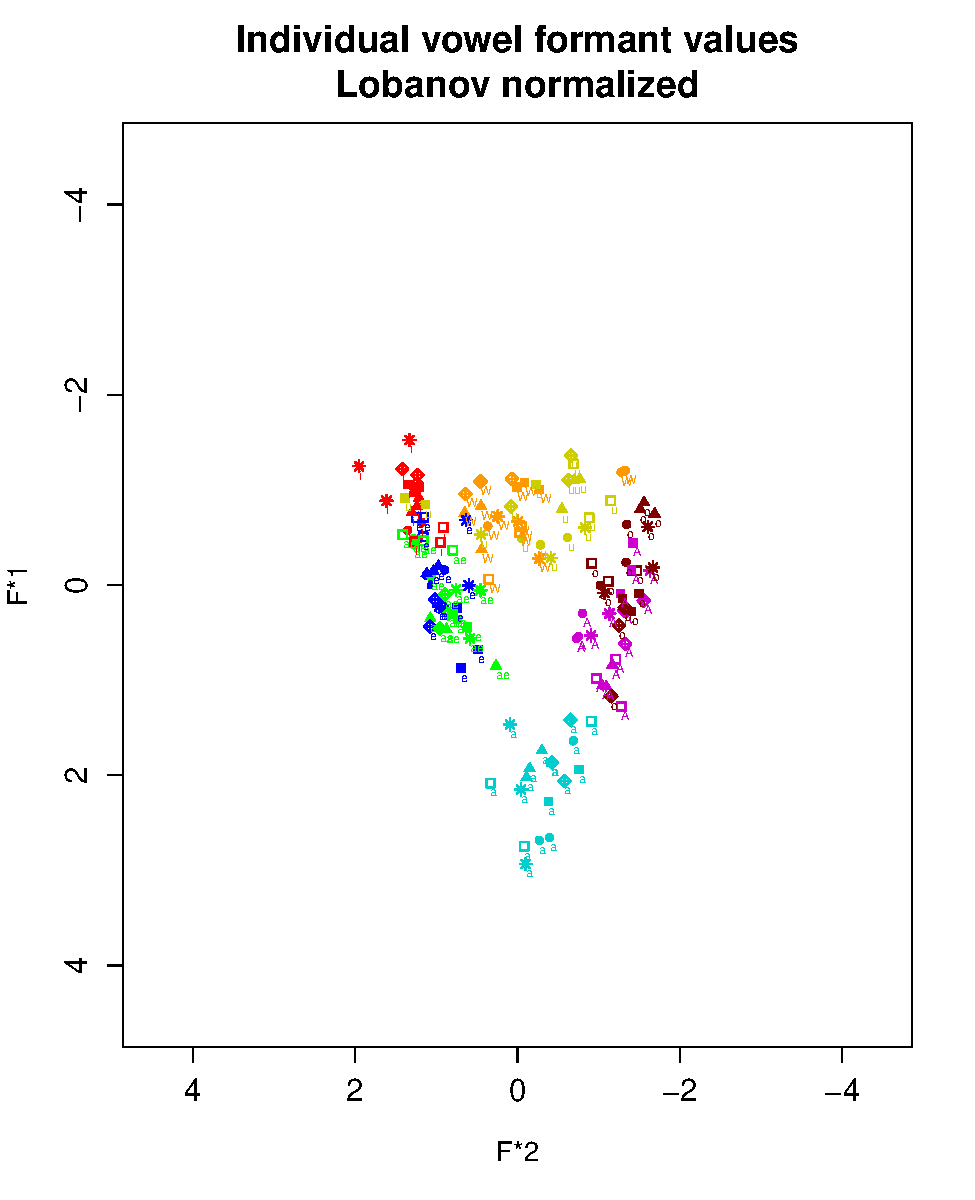
\includegraphics{Group_5_Final_paper_files/figure-latex/SECTION2-1.pdf}
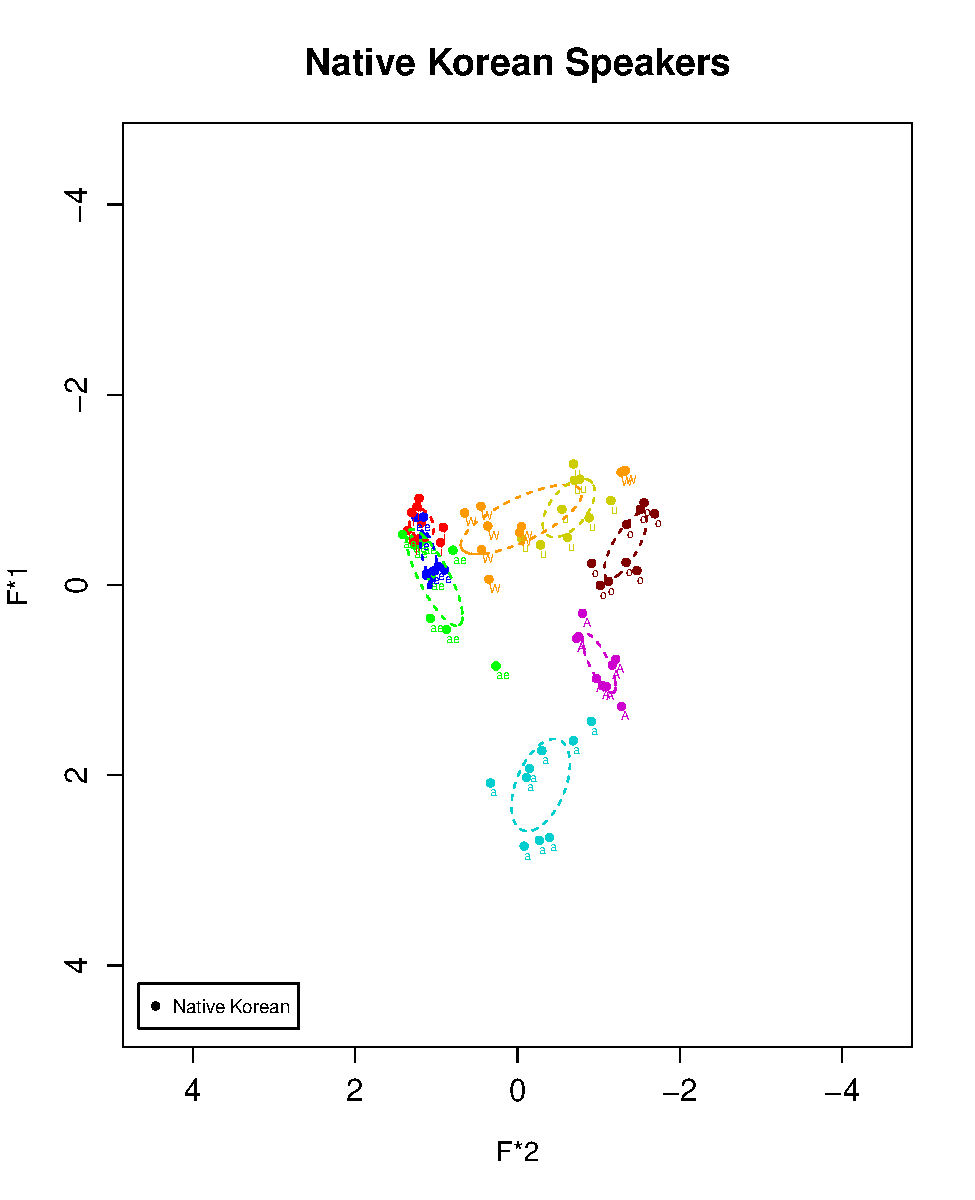
\includegraphics{Group_5_Final_paper_files/figure-latex/SECTION2-2.pdf}
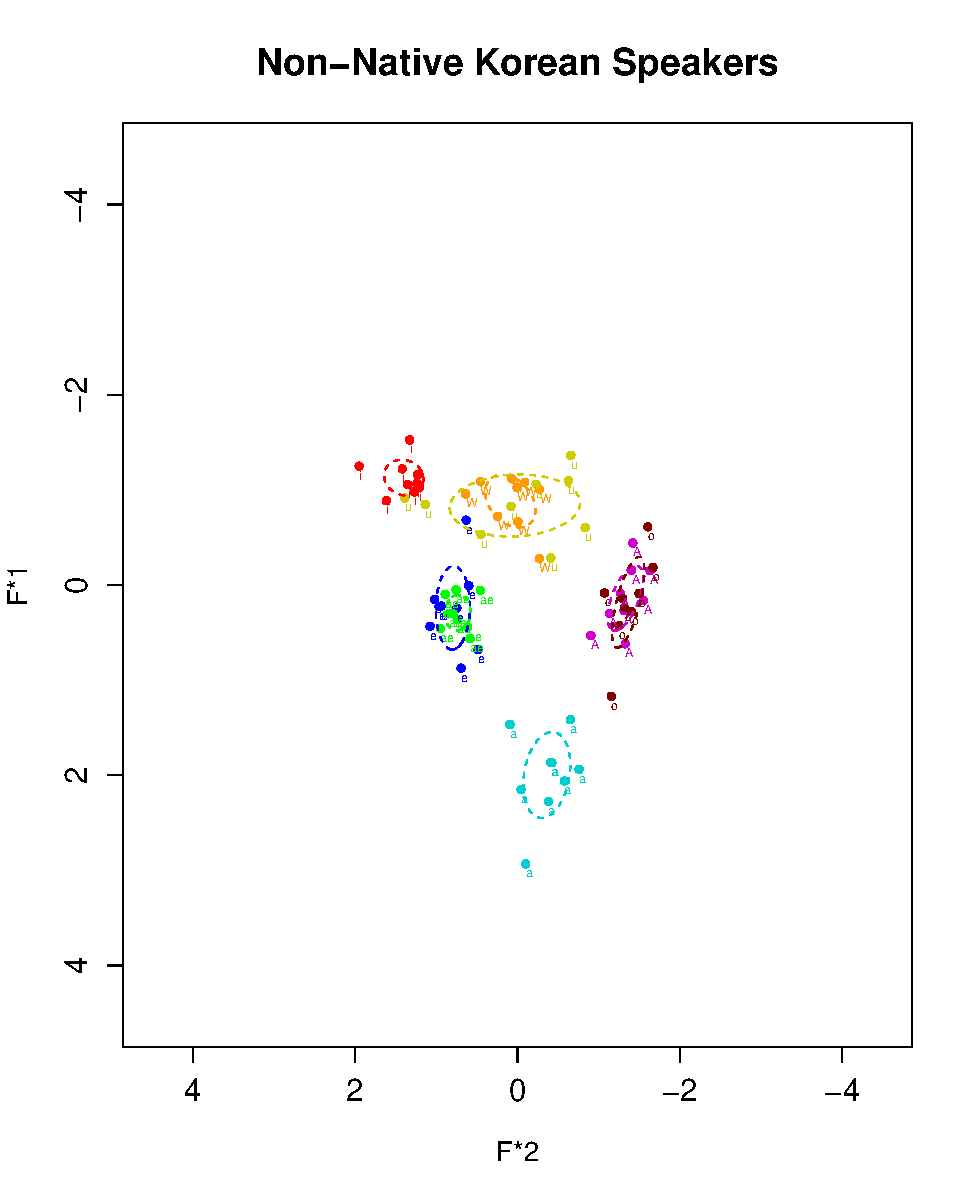
\includegraphics{Group_5_Final_paper_files/figure-latex/SECTION2-3.pdf}
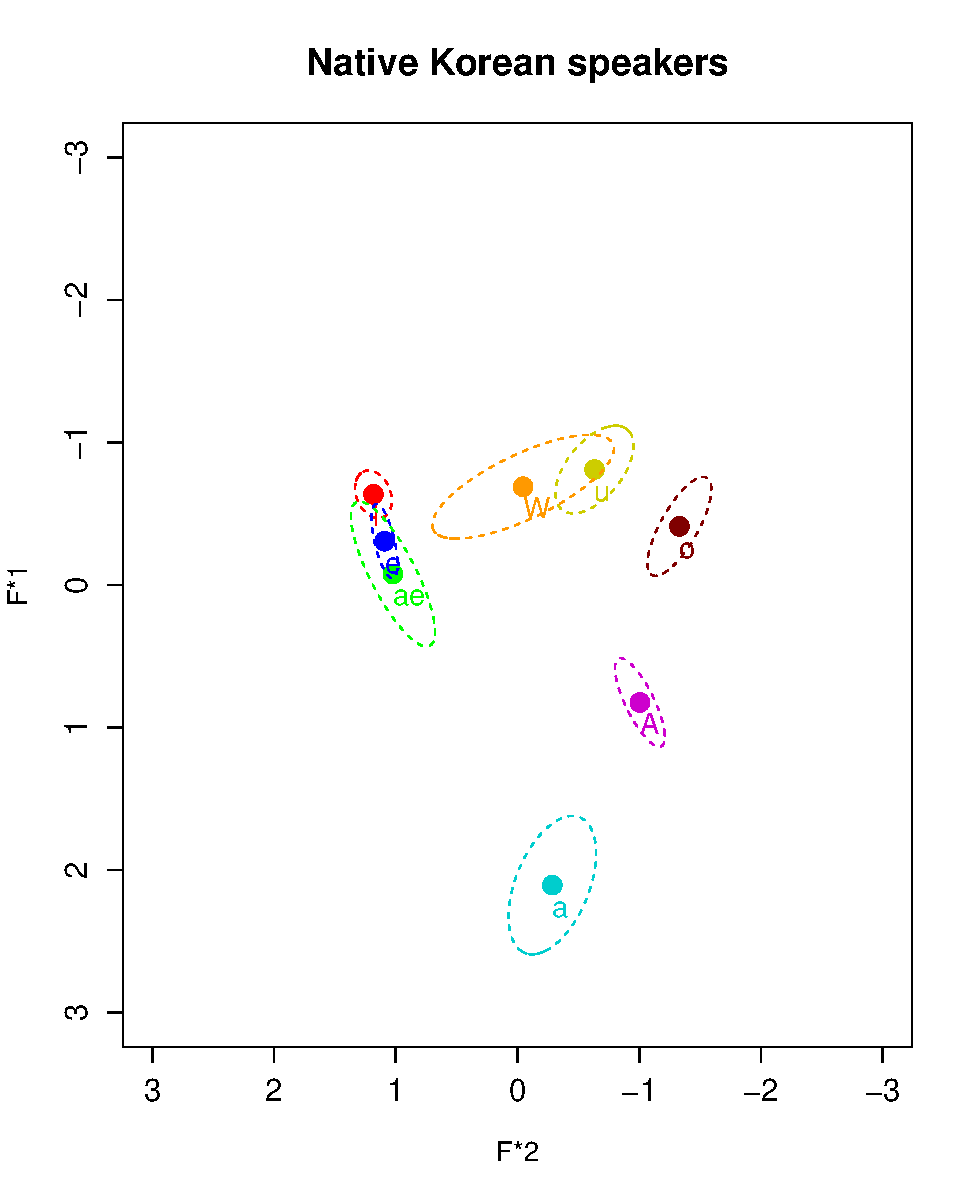
\includegraphics{Group_5_Final_paper_files/figure-latex/SECTION2-4.pdf}
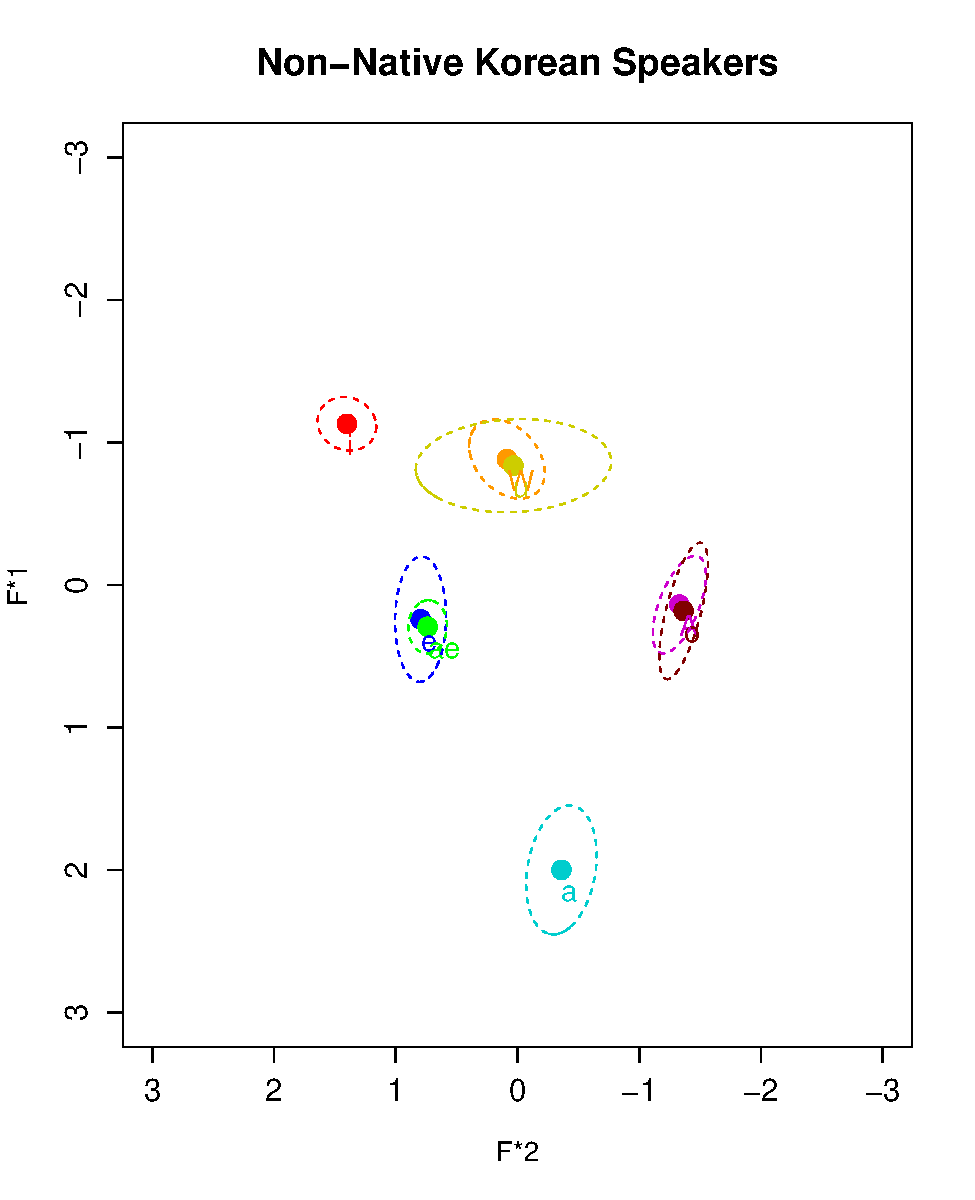
\includegraphics{Group_5_Final_paper_files/figure-latex/SECTION2-5.pdf}
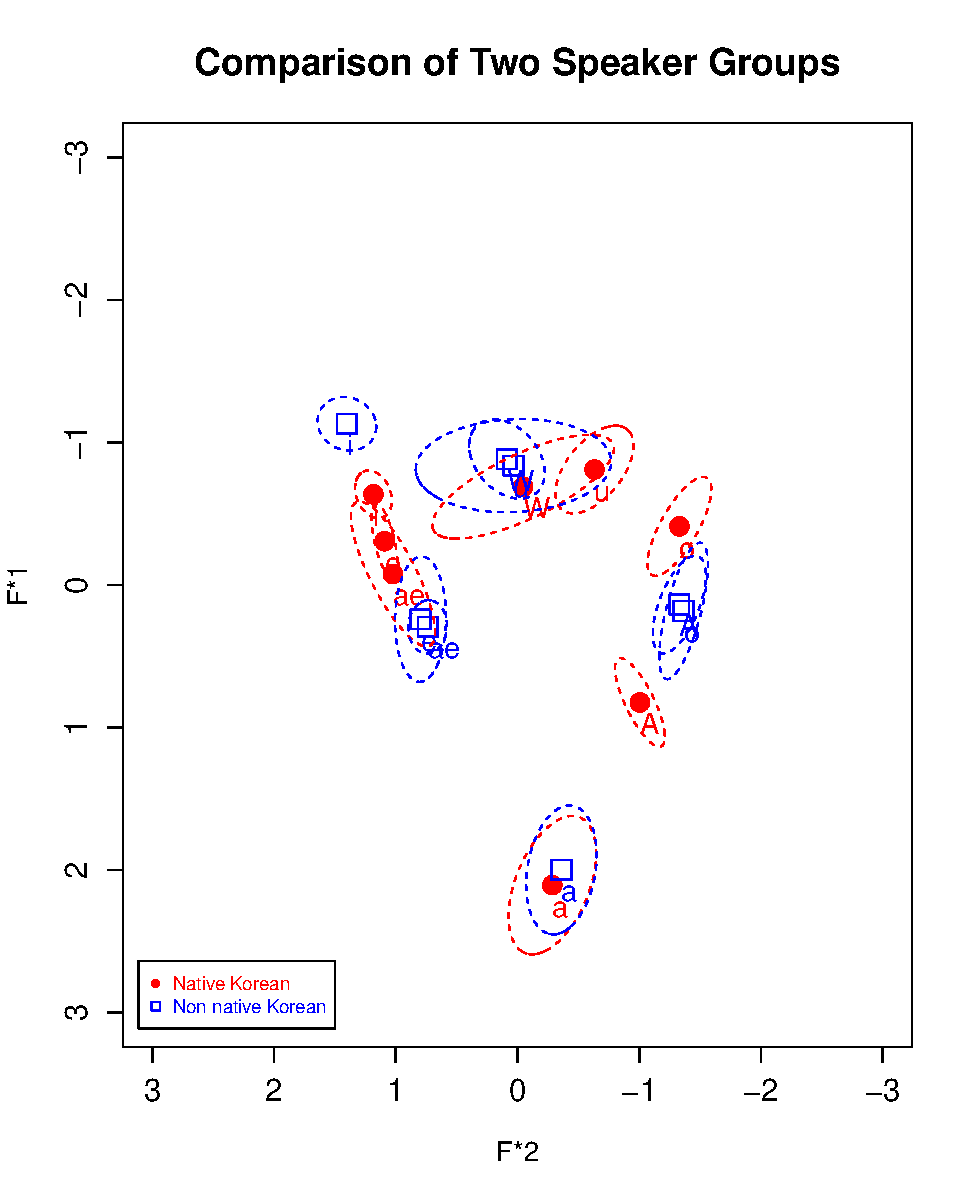
\includegraphics{Group_5_Final_paper_files/figure-latex/SECTION2-6.pdf}

\newpage

\section{\texorpdfstring{\textbf{1.Introduction}}{1.Introduction}}\label{introduction}

In this paper, our group investigated Korean vowel productions of Korean
native speakers (NS) and non-native Korean speakers (NNS) by analyzing
acoustic features. We aimed to examine native speaker pattern of vowel
formants in Korean, and to explore second language learners' patterns in
comparison to those of NNSs. Our results were analyzed by using
normalization and statistic functions in the R program. The results
indicate that L1 (English) of the NNSs might affect their L2 Korean
vowel production. It is important to know what sounds students may have
trouble with and what causes the difficulty in L2 Korean acquisition
Seongmoon (2003) Heoung (1965). Thus, this study is useful in terms of
as well as suggesting crucial research in the second language education
field.

\section{\texorpdfstring{\textbf{2.
Methodology}}{2. Methodology}}\label{methodology}

To compare the convergence and divergence of L1 Korean and L2 Korean
Vowel Production, we used a one-way between-subjects design, and
analyzed the collected data using two Hz-basd measurements and a
phonetic measurement tool, Praat.

\subsection{\texorpdfstring{\emph{2.1
Participants}}{2.1 Participants}}\label{participants}

Using convenince sampling, we sampled six adult residents living in
Eugene, Oregon; three of them were Native Koreans, and the rest were
non-Native sperking Koreans. Two Native Koreans were doctoral students
majoring in East Asian Lanuages and Literatures, and the other one was a
Korean instructor at the University of Oregon. Non-native speakers were
recruited from one of the Korean classes at the Univeresity of Oregon.
Korean participants were an average of 28 in age, while the average age
of the non-Korean subjects were 19.

\subsection{\texorpdfstring{\emph{2.2 Speech
Materials}}{2.2 Speech Materials}}\label{speech-materials}

We prepared seven sentences consisting of eight Korean vowels;
i,e,ae,w,\^{},a,u. The sentences to be tested will be added at the end
of the orignial paper as one of the appendice.

\subsection{\texorpdfstring{\emph{2.3
Procedure}}{2.3 Procedure}}\label{procedure}

The Korean vowles of the participants were audie-recorded. We met in the
quite room individally and we had them repeat the eight sentences three
times using a Praat program, which is widely used in phonetic
measurements. By measuring F1 and F2 in the vowel mid-point, we intended
to find vowel formant patterns.

\section{\texorpdfstring{\textbf{3. Restuls and
Discussion}}{3. Restuls and Discussion}}\label{restuls-and-discussion}

In this section, vowel formant patterns of NSs and NNSs will be
contrasted based on the obtained speech samples. First, we will report
the mean ferments across three repetitions. Namely, the vowel charts all
participants based on mean values will be presented and compared below.
The NS vowel charts reveal several convergences and divergences among
the native speakers. For instance, NS1 tends to pronounce high-back
vowel {[}u{]} as a front vowel. Meanwhile, her high-mid vowel {[}W{]}
also approximates a high back vowel. Another sparkling native speaker is
NS3, who is the only native subject who did not demonstrate a merge of
{[}i{]}, {[}e{]}, and {[}æ{]}, marked by her clear differentiation of
{[}e{]} and {[}æ{]}. In general, NS 3 produced a similar pattern with
the vowel chart of Shin, Kiaer, and Cha (2012) regardless of some subtle
variations. For instance, the mid-back vowel {[}o{]} in Shin et al.
(2012) is realized as a high-back vowel by NS3. NS3's distinction in
vowel articulation might be triggered by multiple reasons. Her standard
Korean training experience for a teaching certificate in the Seoul
Education office, as well as her relative shorter residence in English
speaking countries, might be the causes. In the next section, we will
present the vowel charts of NNS. Several shared typical L2 errors from
the NNS data can be observed. First, compared to the NSs, none of the
NNS participants successfully distinguished {[}A{]} and {[}o{]}.
Although English vowels contrast {[}A{]} and {[}o{]}, due to their
shorter duration of learning Korean (five months), they may not have
fully acquired the accurate L2 pronunciation. Moreover, except for NNS
2, the other two NNSs were both confused between {[}W{]} and {[}u{]}.
Since NS 1 and NS 3 are their teachers in the Korean 102 class, they
might have assimilated teachers' inputs when producing the two sounds.
In addition, given the apparent difference between {[}e{]} of
\enquote{met} and {[}æ{]} of \enquote{mat} in English, they articulated
{[}e{]} and {[}æ{]} as a merged vowel {[}e{]}. In other words, the
merger consistently appeared in the NNS pronunciation because the
teachers might not have fully explained the differences between {[}e{]}
and {[}æ{]}, or the students might not have perceived any
dissimilarities between the teachers' pronunciations. Fortunately, there
are noticeable native-like vowel patterns in the NNSs' data as well.
Especially their accurate production of {[}i{]} and {[}a{]}. They
pronounce {[}i{]} as a high front vowel and {[}a{]} as a low mid vowel.
Since there are similarities between Korean vowels and English vowels--
English {[}i{]} is also articulated in a high front position of the
vocal tract-- they managed to produce Korean vowel {[}i{]} correctly.
However, {[}a{]} has different acoustic features cross-language. For
instance, English does not have {[}a{]} but an {[}a{]}. While the
English {[}a{]} is a low back vowel, the Korean {[}a{]} is a low mid
vowel. Thus, even though Korean {[}a{]} is different from English
{[}a{]}, L2 learners of Korean still can articulate Korean {[}a{]}
accurately. It is interesting that they pronounce {[}a{]} more
native-like than other vowels, despite dissimilarities, which is a
dimension worth thorough investigation in the future analysis.
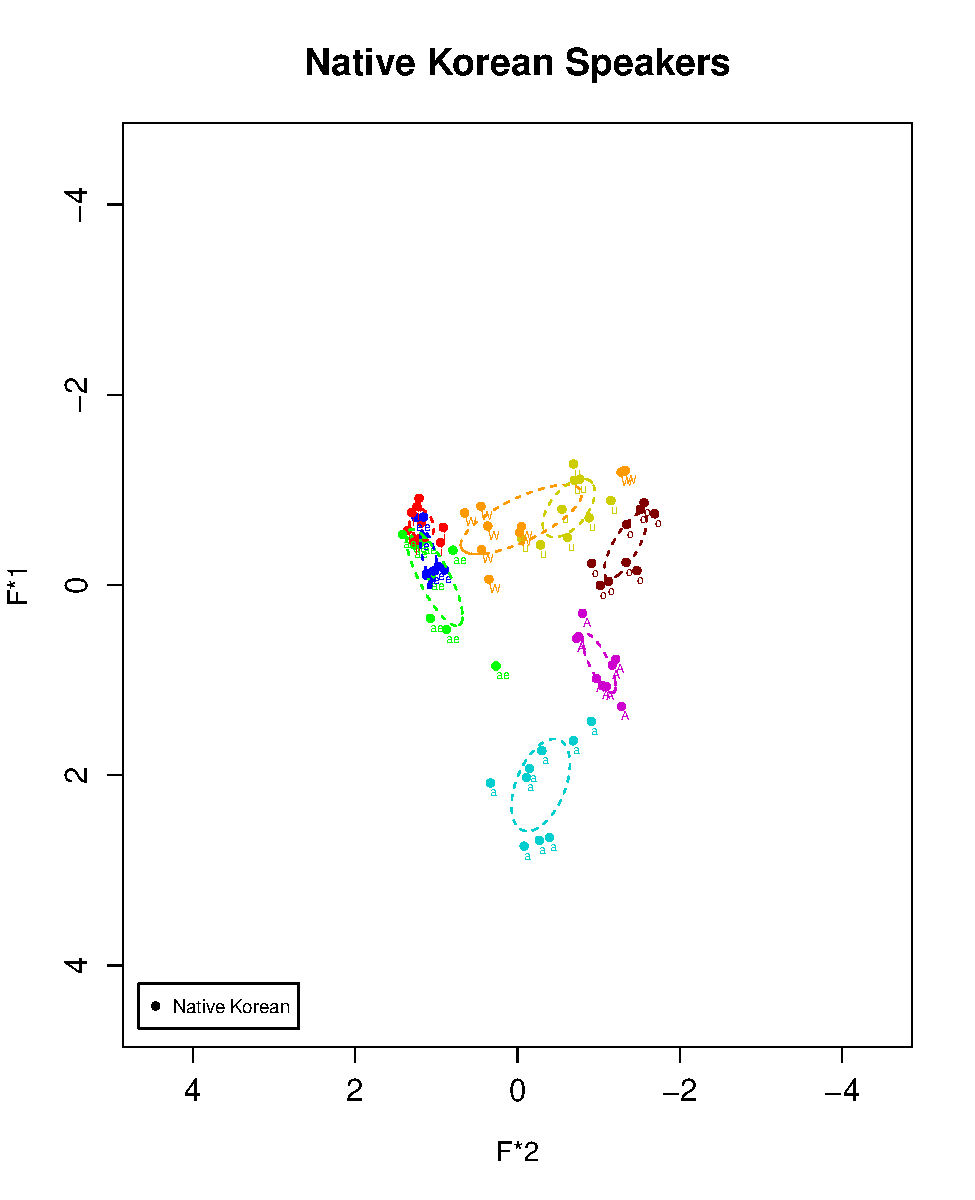
\includegraphics{Group_5_Final_paper_files/figure-latex/Vowel Charts of All Speakers-1.pdf}
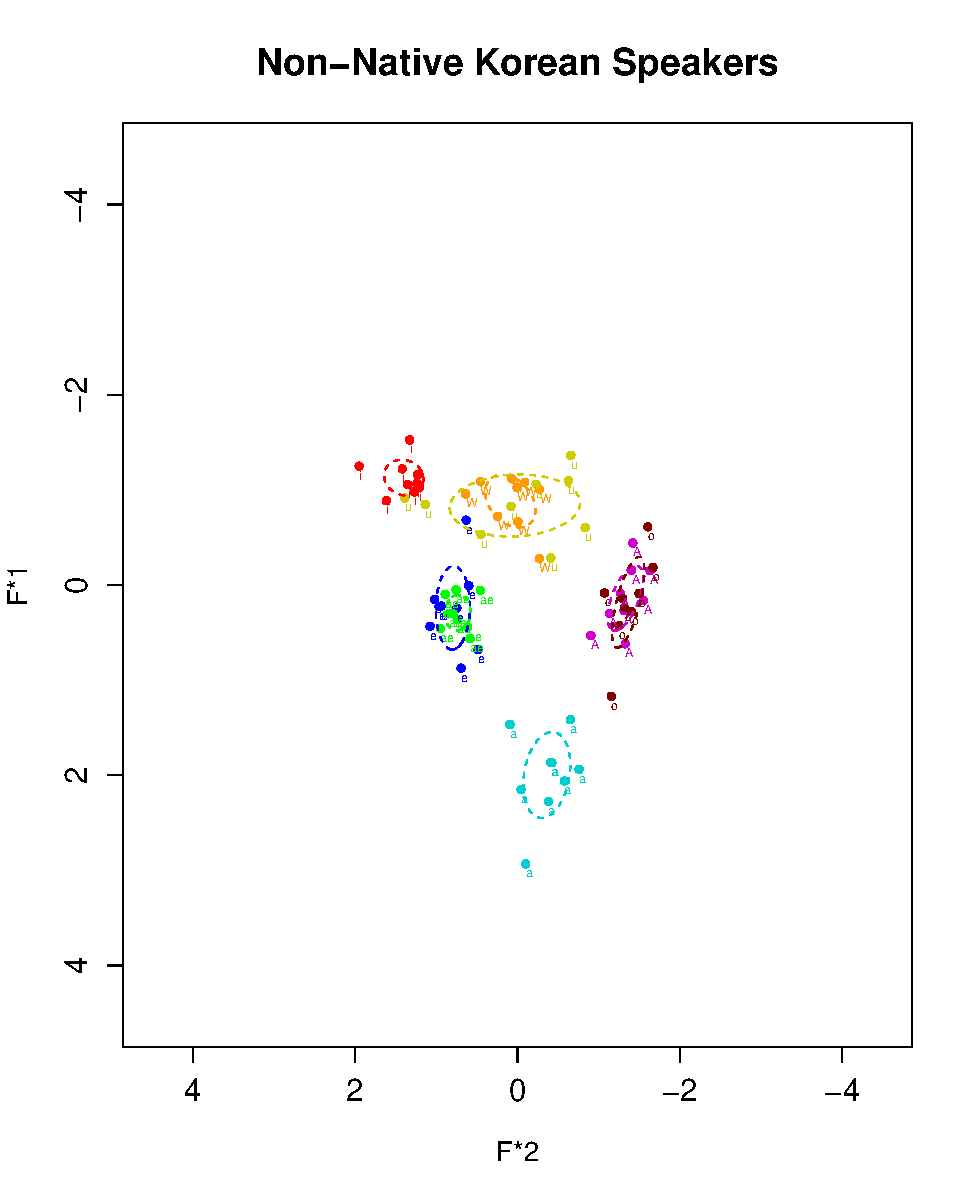
\includegraphics{Group_5_Final_paper_files/figure-latex/Vowel Charts of All Speakers-2.pdf}

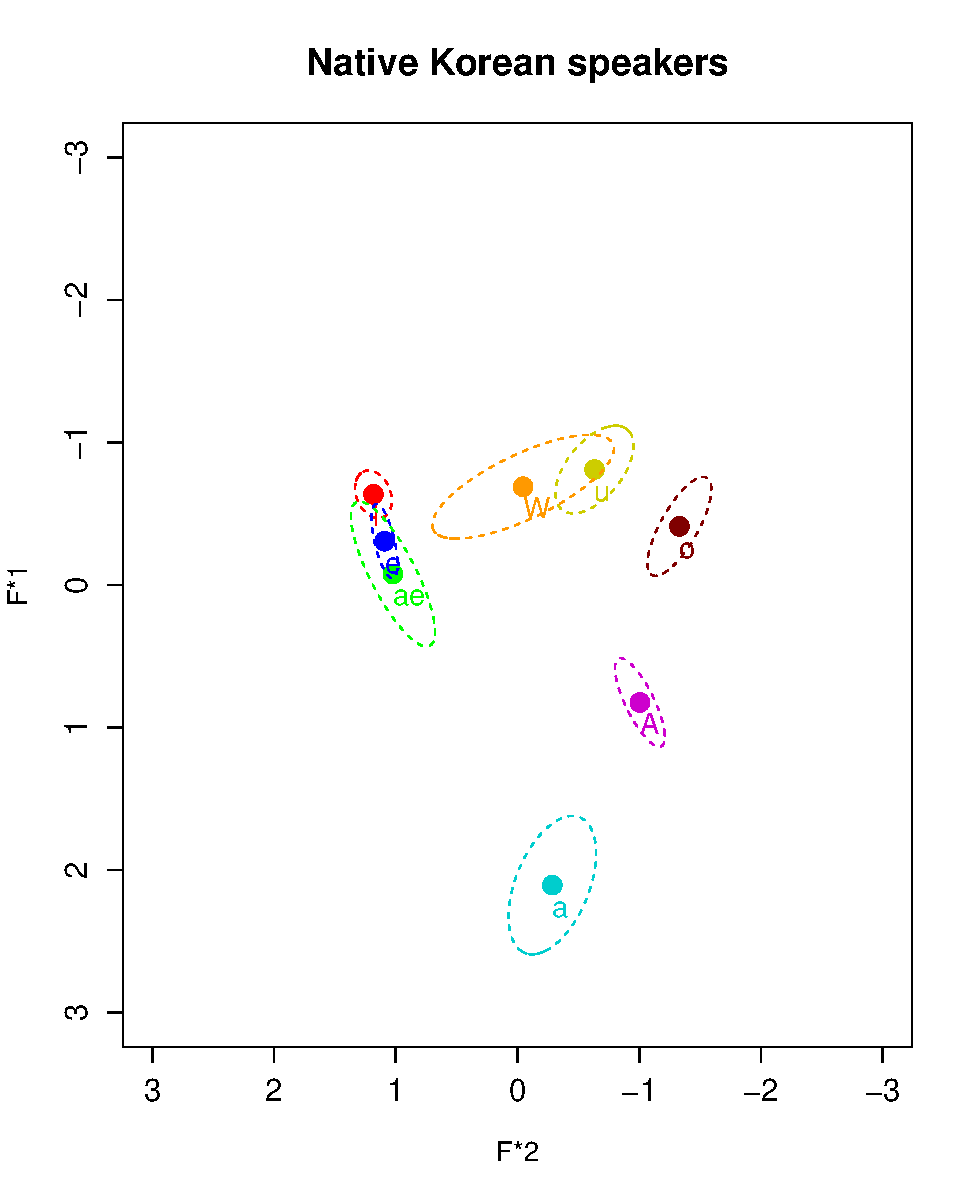
\includegraphics{Group_5_Final_paper_files/figure-latex/Vowel Chart of Mean Values-1.pdf}
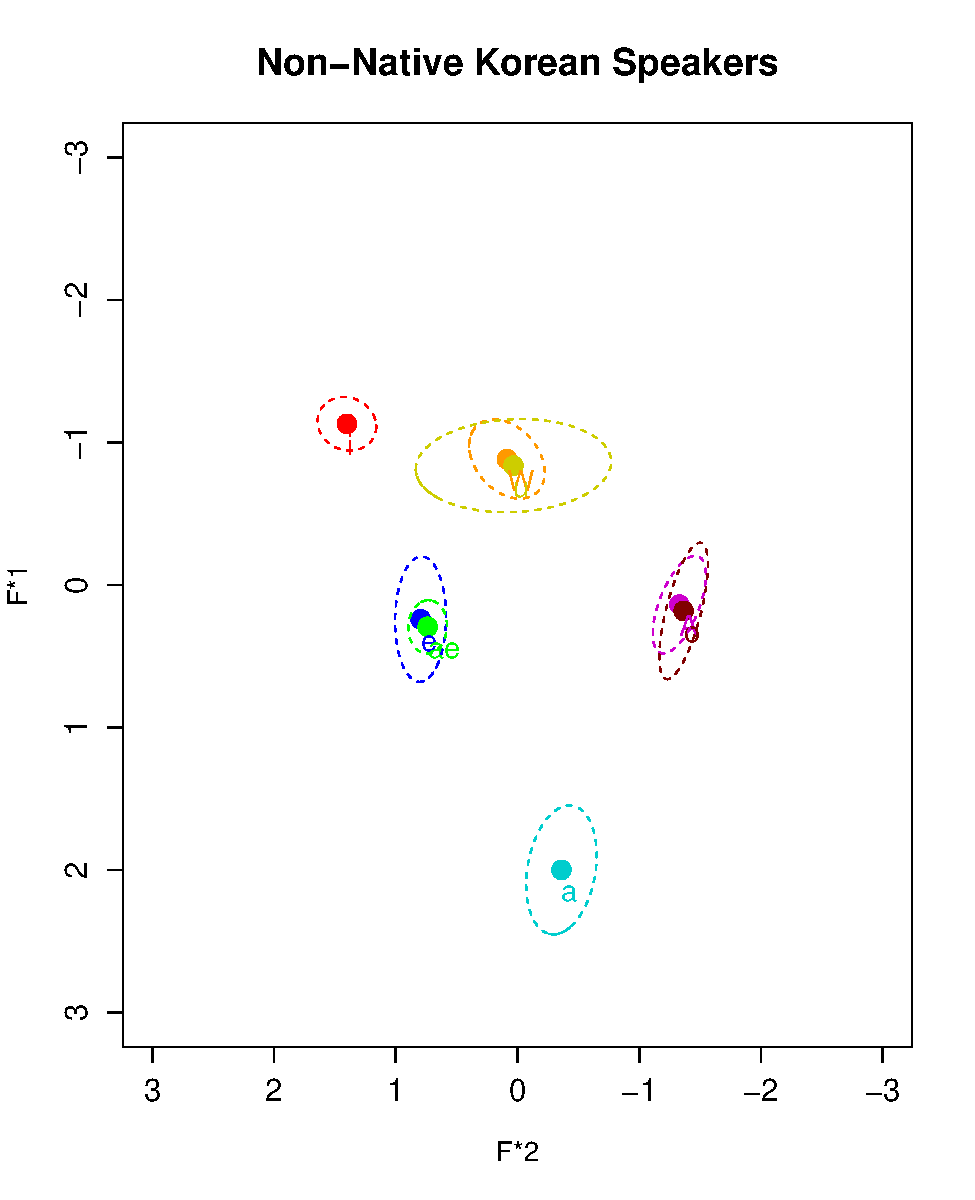
\includegraphics{Group_5_Final_paper_files/figure-latex/Vowel Chart of Mean Values-2.pdf}
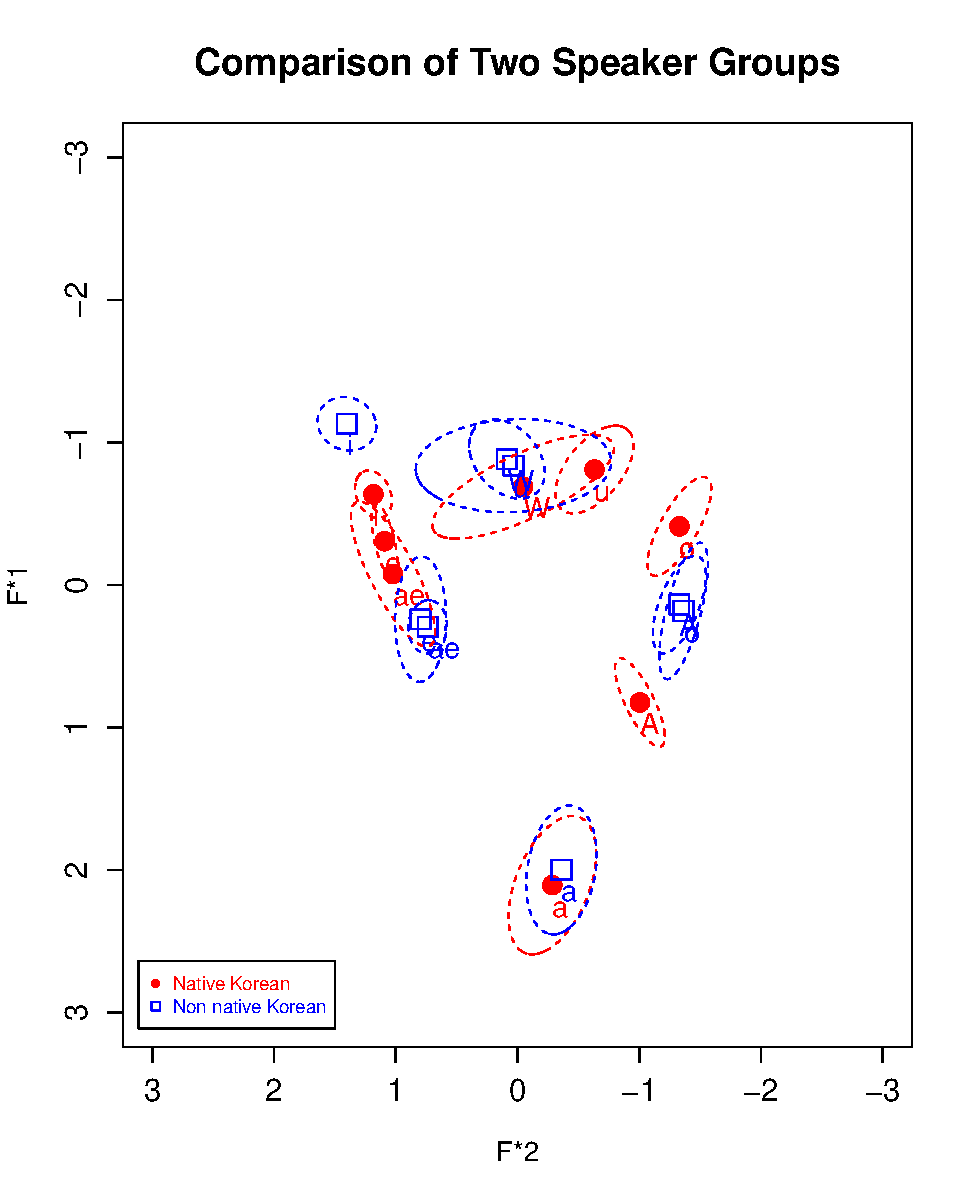
\includegraphics{Group_5_Final_paper_files/figure-latex/Vowel Chart of Mean Values-3.pdf}

\section{\texorpdfstring{\textbf{4.
Conclusion}}{4. Conclusion}}\label{conclusion}

In summary, our analysis indicates that even native Korean speakers may
have different vowel formant patterns due to their various duration of
living in foreign countries and native language phonetic training.
Additionally, teachers' classroom input may play an essential role in L2
sound acquisition. For instance, the NNS in this study demonstrated a
confusion between vowel {[}W{]} and {[}u{]}. Furthermore, despite the
dissimilarities between the participants' L1 and L2, the learners still
can have relatively more native-like articulations of {[}a{]}. We
speculate that the teacher's demo pronunciation and explicit instruction
are critical for this achievement. In the meantime, the vowels {[}e{]}
and {[}æ{]} extracted from the current data are controversial. Since the
merger of {[}e{]} and {[}æ{]} is progressing in Standard Seoul Korean,
how to teach the articulations of these two sounds needs to be discussed
in the future. \newpage

\section{\texorpdfstring{\textbf{5.
Apendix}}{5. Apendix}}\label{apendix}

\begin{tabular}{l|l|l|r|r|l|l|l|l}
\hline
speaker & vowel/frame & context & F1 & F2 & F3 & gl F1 & gl F2 & gl F3\\
\hline
NS1 & i & s & 493.2375 & 2751.1464 & NA & NA & NA & NA\\
\hline
NS1 & i & s & 507.5334 & 2865.6353 & NA & NA & NA & NA\\
\hline
NS1 & i & s & 522.4271 & 2776.4157 & NA & NA & NA & NA\\
\hline
NS1 & e & s & 585.4128 & 2708.4025 & NA & NA & NA & NA\\
\hline
NS1 & e & s & 584.2901 & 2706.7544 & NA & NA & NA & NA\\
\hline
NS1 & e & s & 576.3157 & 2553.8634 & NA & NA & NA & NA\\
\hline
NS1 & ae & s & 521.9904 & 2820.2192 & NA & NA & NA & NA\\
\hline
NS1 & ae & s & 532.9491 & 2809.9055 & NA & NA & NA & NA\\
\hline
NS1 & ae & s & 587.5074 & 2668.7089 & NA & NA & NA & NA\\
\hline
NS1 & W & s & 406.3744 & 1063.7681 & NA & NA & NA & NA\\
\hline
NS1 & W & s & 403.2908 & 1029.0942 & NA & NA & NA & NA\\
\hline
NS1 & W & s & 500.0833 & 2189.0697 & NA & NA & NA & NA\\
\hline
NS1 & A & s & 651.3945 & 1389.8223 & NA & NA & NA & NA\\
\hline
NS1 & A & s & 695.3000 & 1439.2194 & NA & NA & NA & NA\\
\hline
NS1 & A & s & 691.9308 & 1425.3407 & NA & NA & NA & NA\\
\hline
NS1 & a & s & 1040.9052 & 1666.9375 & NA & NA & NA & NA\\
\hline
NS1 & a & s & 872.9430 & 1467.5644 & NA & NA & NA & NA\\
\hline
NS1 & a & s & 1045.7113 & 1754.2864 & NA & NA & NA & NA\\
\hline
NS1 & u & s & 532.7743 & 1744.8213 & NA & NA & NA & NA\\
\hline
NS1 & u & s & 521.8414 & 1904.3388 & NA & NA & NA & NA\\
\hline
NS1 & u & s & 519.8707 & 1516.3195 & NA & NA & NA & NA\\
\hline
NS1 & o & s & 497.1905 & 1015.9893 & NA & NA & NA & NA\\
\hline
NS1 & o & s & 603.1489 & 1240.2403 & NA & NA & NA & NA\\
\hline
NS1 & o & s & 563.1774 & 1021.5937 & NA & NA & NA & NA\\
\hline
NS2 & i & s & 484.5754 & 2530.1916 & NA & NA & NA & NA\\
\hline
NS2 & i & s & 506.4917 & 2749.4107 & NA & NA & NA & NA\\
\hline
NS2 & i & s & 507.1835 & 2551.5501 & NA & NA & NA & NA\\
\hline
NS2 & e & s & 469.0207 & 2680.1408 & NA & NA & NA & NA\\
\hline
NS2 & e & s & 498.8255 & 2682.3309 & NA & NA & NA & NA\\
\hline
NS2 & e & s & 470.0572 & 2737.2926 & NA & NA & NA & NA\\
\hline
NS2 & ae & s & 504.6131 & 2682.5265 & NA & NA & NA & NA\\
\hline
NS2 & ae & s & 518.9117 & 2455.7005 & NA & NA & NA & NA\\
\hline
NS2 & ae & s & 495.4734 & 2840.3980 & NA & NA & NA & NA\\
\hline
NS2 & W & s & 562.5110 & 2181.1447 & NA & NA & NA & NA\\
\hline
NS2 & W & s & 483.4509 & 1934.0088 & NA & NA & NA & NA\\
\hline
NS2 & W & s & 492.3308 & 1946.6732 & NA & NA & NA & NA\\
\hline
NS2 & A & s & 753.6069 & 1168.1896 & NA & NA & NA & NA\\
\hline
NS2 & A & s & 711.6761 & 1359.5595 & NA & NA & NA & NA\\
\hline
NS2 & A & s & 682.6742 & 1211.4757 & NA & NA & NA & NA\\
\hline
NS2 & a & s & 868.5899 & 2169.0841 & NA & NA & NA & NA\\
\hline
NS2 & a & s & 963.4477 & 1911.3544 & NA & NA & NA & NA\\
\hline
NS2 & a & s & 776.1289 & 1397.6685 & NA & NA & NA & NA\\
\hline
NS2 & u & s & 444.4061 & 1247.9899 & NA & NA & NA & NA\\
\hline
NS2 & u & s & 389.3091 & 1533.5457 & NA & NA & NA & NA\\
\hline
NS2 & u & s & 470.3084 & 1413.8744 & NA & NA & NA & NA\\
\hline
NS2 & o & s & 549.6220 & 1049.1350 & NA & NA & NA & NA\\
\hline
NS2 & o & s & 565.7779 & 1267.5317 & NA & NA & NA & NA\\
\hline
NS2 & o & s & 538.5363 & 1395.5907 & NA & NA & NA & NA\\
\hline
NS3 & i & s & 387.8858 & 2396.4313 & NA & NA & NA & NA\\
\hline
NS3 & i & s & 372.6968 & 2362.0638 & NA & NA & NA & NA\\
\hline
NS3 & i & s & 351.5644 & 2349.0573 & NA & NA & NA & NA\\
\hline
NS3 & e & s & 541.6388 & 2299.6618 & NA & NA & NA & NA\\
\hline
NS3 & e & s & 522.9438 & 2222.9239 & NA & NA & NA & NA\\
\hline
NS3 & e & s & 534.8824 & 2255.4659 & NA & NA & NA & NA\\
\hline
NS3 & ae & s & 682.1858 & 2171.0594 & NA & NA & NA & NA\\
\hline
NS3 & ae & s & 773.9753 & 1849.0509 & NA & NA & NA & NA\\
\hline
NS3 & ae & s & 653.9953 & 2275.9436 & NA & NA & NA & NA\\
\hline
NS3 & W & s & 371.8679 & 1946.9052 & NA & NA & NA & NA\\
\hline
NS3 & W & s & 388.4859 & 2052.6352 & NA & NA & NA & NA\\
\hline
NS3 & W & s & 480.6599 & 1942.7974 & NA & NA & NA & NA\\
\hline
NS3 & A & s & 771.6552 & 1094.0478 & NA & NA & NA & NA\\
\hline
NS3 & A & s & 826.2665 & 1132.6897 & NA & NA & NA & NA\\
\hline
NS3 & A & s & 823.3914 & 1158.7672 & NA & NA & NA & NA\\
\hline
NS3 & a & s & 1054.9720 & 1650.8194 & NA & NA & NA & NA\\
\hline
NS3 & a & s & 1032.3468 & 1631.0017 & NA & NA & NA & NA\\
\hline
NS3 & a & s & 987.4001 & 1551.0025 & NA & NA & NA & NA\\
\hline
NS3 & u & s & 379.3075 & 1421.1645 & NA & NA & NA & NA\\
\hline
NS3 & u & s & 303.4930 & 1305.0793 & NA & NA & NA & NA\\
\hline
NS3 & u & s & 306.2061 & 1340.5713 & NA & NA & NA & NA\\
\hline
NS3 & o & s & 390.7935 & 818.3821 & NA & NA & NA & NA\\
\hline
NS3 & o & s & 362.6956 & 886.9867 & NA & NA & NA & NA\\
\hline
NS3 & o & s & 379.7458 & 911.8159 & NA & NA & NA & NA\\
\hline
\end{tabular}

\begin{tabular}{l|l|l|r|r|l|l|l|l}
\hline
speaker & vowel/frame & context & F1 & F2 & F3 & gl F1 & gl F2 & gl F3\\
\hline
NNS1 & i & s & 347.0051 & 2656.345 & NA & NA & NA & NA\\
\hline
NNS1 & i & s & 399.5299 & 2514.290 & NA & NA & NA & NA\\
\hline
NNS1 & i & s & 307.0789 & 2393.816 & NA & NA & NA & NA\\
\hline
NNS1 & e & s & 560.6831 & 2240.837 & NA & NA & NA & NA\\
\hline
NNS1 & e & s & 528.4257 & 2086.393 & NA & NA & NA & NA\\
\hline
NNS1 & e & s & 429.0911 & 2100.116 & NA & NA & NA & NA\\
\hline
NNS1 & ae & s & 534.9859 & 2152.606 & NA & NA & NA & NA\\
\hline
NNS1 & ae & s & 609.0134 & 2080.387 & NA & NA & NA & NA\\
\hline
NNS1 & ae & s & 535.6872 & 2026.094 & NA & NA & NA & NA\\
\hline
NNS1 & W & s & 487.4876 & 1719.508 & NA & NA & NA & NA\\
\hline
NNS1 & W & s & 423.2244 & 1936.019 & NA & NA & NA & NA\\
\hline
NNS1 & W & s & 431.3064 & 1830.811 & NA & NA & NA & NA\\
\hline
NNS1 & A & s & 604.5336 & 1451.755 & NA & NA & NA & NA\\
\hline
NNS1 & A & s & 505.9047 & 1144.177 & NA & NA & NA & NA\\
\hline
NNS1 & A & s & 571.0737 & 1355.492 & NA & NA & NA & NA\\
\hline
NNS1 & a & s & 951.4490 & 1789.920 & NA & NA & NA & NA\\
\hline
NNS1 & a & s & 838.7338 & 1815.066 & NA & NA & NA & NA\\
\hline
NNS1 & a & s & 739.6891 & 1872.772 & NA & NA & NA & NA\\
\hline
NNS1 & u & s & 440.4063 & 1481.121 & NA & NA & NA & NA\\
\hline
NNS1 & u & s & 486.5747 & 1659.796 & NA & NA & NA & NA\\
\hline
NNS1 & u & s & 450.5802 & 2023.228 & NA & NA & NA & NA\\
\hline
NNS1 & o & s & 539.7927 & 1380.349 & NA & NA & NA & NA\\
\hline
NNS1 & o & s & 501.0599 & 1128.311 & NA & NA & NA & NA\\
\hline
NNS1 & o & s & 439.2177 & 1155.855 & NA & NA & NA & NA\\
\hline
NNS2 & i & s & 361.5158 & 2606.105 & NA & NA & NA & NA\\
\hline
NNS2 & i & s & 345.7214 & 2602.082 & NA & NA & NA & NA\\
\hline
NNS2 & i & s & 334.6823 & 2699.489 & NA & NA & NA & NA\\
\hline
NNS2 & e & s & 623.4945 & 2523.746 & NA & NA & NA & NA\\
\hline
NNS2 & e & s & 586.4921 & 2453.199 & NA & NA & NA & NA\\
\hline
NNS2 & e & s & 574.2458 & 2494.539 & NA & NA & NA & NA\\
\hline
NNS2 & ae & s & 627.4423 & 2460.190 & NA & NA & NA & NA\\
\hline
NNS2 & ae & s & 565.0315 & 2428.970 & NA & NA & NA & NA\\
\hline
NNS2 & ae & s & 600.7081 & 2407.691 & NA & NA & NA & NA\\
\hline
NNS2 & W & s & 353.2532 & 2007.973 & NA & NA & NA & NA\\
\hline
NNS2 & W & s & 357.8650 & 2206.426 & NA & NA & NA & NA\\
\hline
NNS2 & W & s & 380.6912 & 2300.526 & NA & NA & NA & NA\\
\hline
NNS2 & A & s & 655.8457 & 1293.970 & NA & NA & NA & NA\\
\hline
NNS2 & A & s & 576.4614 & 1177.686 & NA & NA & NA & NA\\
\hline
NNS2 & A & s & 595.1642 & 1301.263 & NA & NA & NA & NA\\
\hline
NNS2 & a & s & 873.8260 & 1756.333 & NA & NA & NA & NA\\
\hline
NNS2 & a & s & 907.4390 & 1677.641 & NA & NA & NA & NA\\
\hline
NNS2 & a & s & 794.9709 & 1639.282 & NA & NA & NA & NA\\
\hline
NNS2 & u & s & 355.8018 & 1651.668 & NA & NA & NA & NA\\
\hline
NNS2 & u & s & 403.5285 & 2013.179 & NA & NA & NA & NA\\
\hline
NNS2 & u & s & 310.0982 & 1636.685 & NA & NA & NA & NA\\
\hline
NNS2 & o & s & 752.1455 & 1381.457 & NA & NA & NA & NA\\
\hline
NNS2 & o & s & 622.5061 & 1332.064 & NA & NA & NA & NA\\
\hline
NNS2 & o & s & 589.4089 & 1297.657 & NA & NA & NA & NA\\
\hline
NNS3 & i & s & 406.4256 & 2437.481 & NA & NA & NA & NA\\
\hline
NNS3 & i & s & 402.6381 & 2509.160 & NA & NA & NA & NA\\
\hline
NNS3 & i & s & 411.3147 & 2467.863 & NA & NA & NA & NA\\
\hline
NNS3 & e & s & 551.3395 & 2200.921 & NA & NA & NA & NA\\
\hline
NNS3 & e & s & 601.2305 & 2067.347 & NA & NA & NA & NA\\
\hline
NNS3 & e & s & 623.6768 & 2174.703 & NA & NA & NA & NA\\
\hline
NNS3 & ae & s & 558.3153 & 2224.343 & NA & NA & NA & NA\\
\hline
NNS3 & ae & s & 565.0498 & 2198.490 & NA & NA & NA & NA\\
\hline
NNS3 & ae & s & 574.3903 & 2133.683 & NA & NA & NA & NA\\
\hline
NNS3 & W & s & 399.7760 & 1774.814 & NA & NA & NA & NA\\
\hline
NNS3 & W & s & 408.5535 & 1681.144 & NA & NA & NA & NA\\
\hline
NNS3 & W & s & 405.6927 & 1823.001 & NA & NA & NA & NA\\
\hline
NNS3 & A & s & 533.9606 & 1173.059 & NA & NA & NA & NA\\
\hline
NNS3 & A & s & 505.6020 & 1103.150 & NA & NA & NA & NA\\
\hline
NNS3 & A & s & 472.8930 & 1094.922 & NA & NA & NA & NA\\
\hline
NNS3 & a & s & 784.3184 & 1625.894 & NA & NA & NA & NA\\
\hline
NNS3 & a & s & 737.0584 & 1611.615 & NA & NA & NA & NA\\
\hline
NNS3 & a & s & 745.4881 & 1433.147 & NA & NA & NA & NA\\
\hline
NNS3 & u & s & 426.4732 & 2399.924 & NA & NA & NA & NA\\
\hline
NNS3 & u & s & 418.7526 & 2528.042 & NA & NA & NA & NA\\
\hline
NNS3 & u & s & 402.1671 & 1703.117 & NA & NA & NA & NA\\
\hline
NNS3 & o & s & 533.8399 & 1056.215 & NA & NA & NA & NA\\
\hline
NNS3 & o & s & 539.7537 & 1159.086 & NA & NA & NA & NA\\
\hline
NNS3 & o & s & 555.5259 & 1103.115 & NA & NA & NA & NA\\
\hline
\end{tabular}

\section{\texorpdfstring{\textbf{References}}{References}}\label{references}

\begingroup
\setlength{\parindent}{-0.5in} \setlength{\leftskip}{0.5in}

\hypertarget{refs}{}
\hypertarget{ref-Heo1965}{}
Heoung. (1965). Korean phonetics.

\hypertarget{ref-Cho2003}{}
Seongmoon, C. (2003). Acoustic phonetics on the vowel system of modern
korean. \emph{Korean Language and Culture}, \emph{24}, 427--441.

\hypertarget{ref-Shin2012}{}
Shin, J., Kiaer, J., \& Cha, J. (2012). \emph{The sounds of korean}.
Cambridge University Press.

\endgroup


\end{document}
